\section{Results and Discussion}
\label{sec:results}

All results below are drawn directly from
\texttt{results/summary\_table.csv}, \texttt{results/statistical\_tests.csv},
and \texttt{results/fuzzy\_sensitivity\_table.csv}, produced by the 50-run
Monte Carlo sweep described in Section~\ref{sec:scenarios} (19,260 raw
metric rows for the five core algorithms plus a further 7,700 rows for the
fuzzy rule-base sensitivity variants).

\subsection{Steady-State Performance}
Table~\ref{tab:steady-state} summarizes tracking efficiency, steady-state
oscillation, and energy yield ratio at STC (1000\,W/m$^2$, 25\textdegree
C). A one-way ANOVA across the five algorithms is significant for both
tracking efficiency ($F=11.65$, $p=1.12\times10^{-8}$, $\eta^2=0.160$) and
steady-state oscillation ($F=21.88$, $p=1.87\times10^{-15}$,
$\eta^2=0.263$); a Friedman test~\cite{friedman1937use} -- the rank-based,
repeated-measures companion to the ANOVA that exploits the identical-seed
pairing across algorithms directly, rather than treating the five groups
as independent samples -- agrees for both metrics ($\chi^2=177.30$,
$p=2.84\times10^{-37}$ and $\chi^2=79.29$, $p=2.46\times10^{-16}$
respectively, $n=50$ complete runs). Paired $t$-tests (paired by run, per
Section~\ref{sec:scenarios}'s identical-seed design, Holm-Bonferroni-adjusted~\cite{holm1979simple}
within each metric's 10 pairwise comparisons) confirm SMC's tracking
efficiency is significantly higher than every other algorithm's (vs.\
P\&O: $t=-5.11$, $p_{\text{Holm}}=4.7\times10^{-5}$, Cohen's~\cite{cohen1988statistical} $d=-0.72$;
vs.\ fuzzy logic: $t=-4.09$, $p_{\text{Holm}}=8.1\times10^{-4}$, $d=-0.58$;
vs.\ IncCond: $t=-5.05$, $p_{\text{Holm}}=4.9\times10^{-5}$, $d=-0.71$;
vs.\ Q-learning: $t=-3.63$, $p_{\text{Holm}}=2.7\times10^{-3}$, $d=-0.51$)
-- medium-to-large paired effect sizes by convention, not just
statistically detectable ones -- and also has the lowest steady-state
oscillation of all five.

\begin{table}[htbp]
\centering
\caption{Steady-State Performance (Mean $\pm$ Std, $n=50$)}
\label{tab:steady-state}
\begin{tabular}{@{}lccc@{}}
\toprule
Algorithm & Tracking Eff.\ (\%) & Oscillation p2p (W) & Energy Ratio \\
\midrule
P\&O         & $99.73 \pm 0.36$  & $3.38 \pm 1.01$ & $0.9973 \pm 0.0036$ \\
IncCond      & $97.64 \pm 3.29$  & $4.43 \pm 1.18$ & $0.9764 \pm 0.0329$ \\
Fuzzy Logic  & $99.87 \pm 0.18$  & $3.14 \pm 1.11$ & $0.9987 \pm 0.0018$ \\
Q-learning\textsuperscript{a} & $91.84 \pm 15.70$ & $2.88 \pm 1.75$ & $0.9184 \pm 0.1570$ \\
SMC          & $\mathbf{99.90 \pm 0.12}$ & $\mathbf{2.07 \pm 1.29}$ & $\mathbf{0.9990 \pm 0.0012}$ \\
\bottomrule
\multicolumn{4}{l}{\footnotesize\textsuperscript{a}Training-distribution scenario for Q-learning (see \ref{sec:ql-tagging}).} \\
\end{tabular}
\end{table}

Q-learning's own training-distribution performance at steady state is
notably more variable than the other four algorithms ($\sigma=15.70$
versus $\le3.29$ for every other algorithm) -- this is not simply a
held-out generalization gap, since steady-state is itself a
training-distribution scenario. Its \emph{convergence rate} at steady
state is 80\% (40 of 50 runs), versus 100\% for P\&O, fuzzy logic, and SMC
and 70\% for IncCond (Table~\ref{tab:convergence}); this should be reported
alongside the held-out numbers below rather than only the generalization
gap, since it shows the tabular policy does not fully solve even its own
training scenario.

Fig.~\ref{fig:metric-comparison} shows tracking efficiency across all
eleven scenarios; the two-line caption reflects that Q-learning's bars
represent held-out (untrained) conditions except at steady-state and
step-change-irradiance, per Section~\ref{sec:ql-tagging}'s tagging.

\begin{figure}[htbp]
\centering
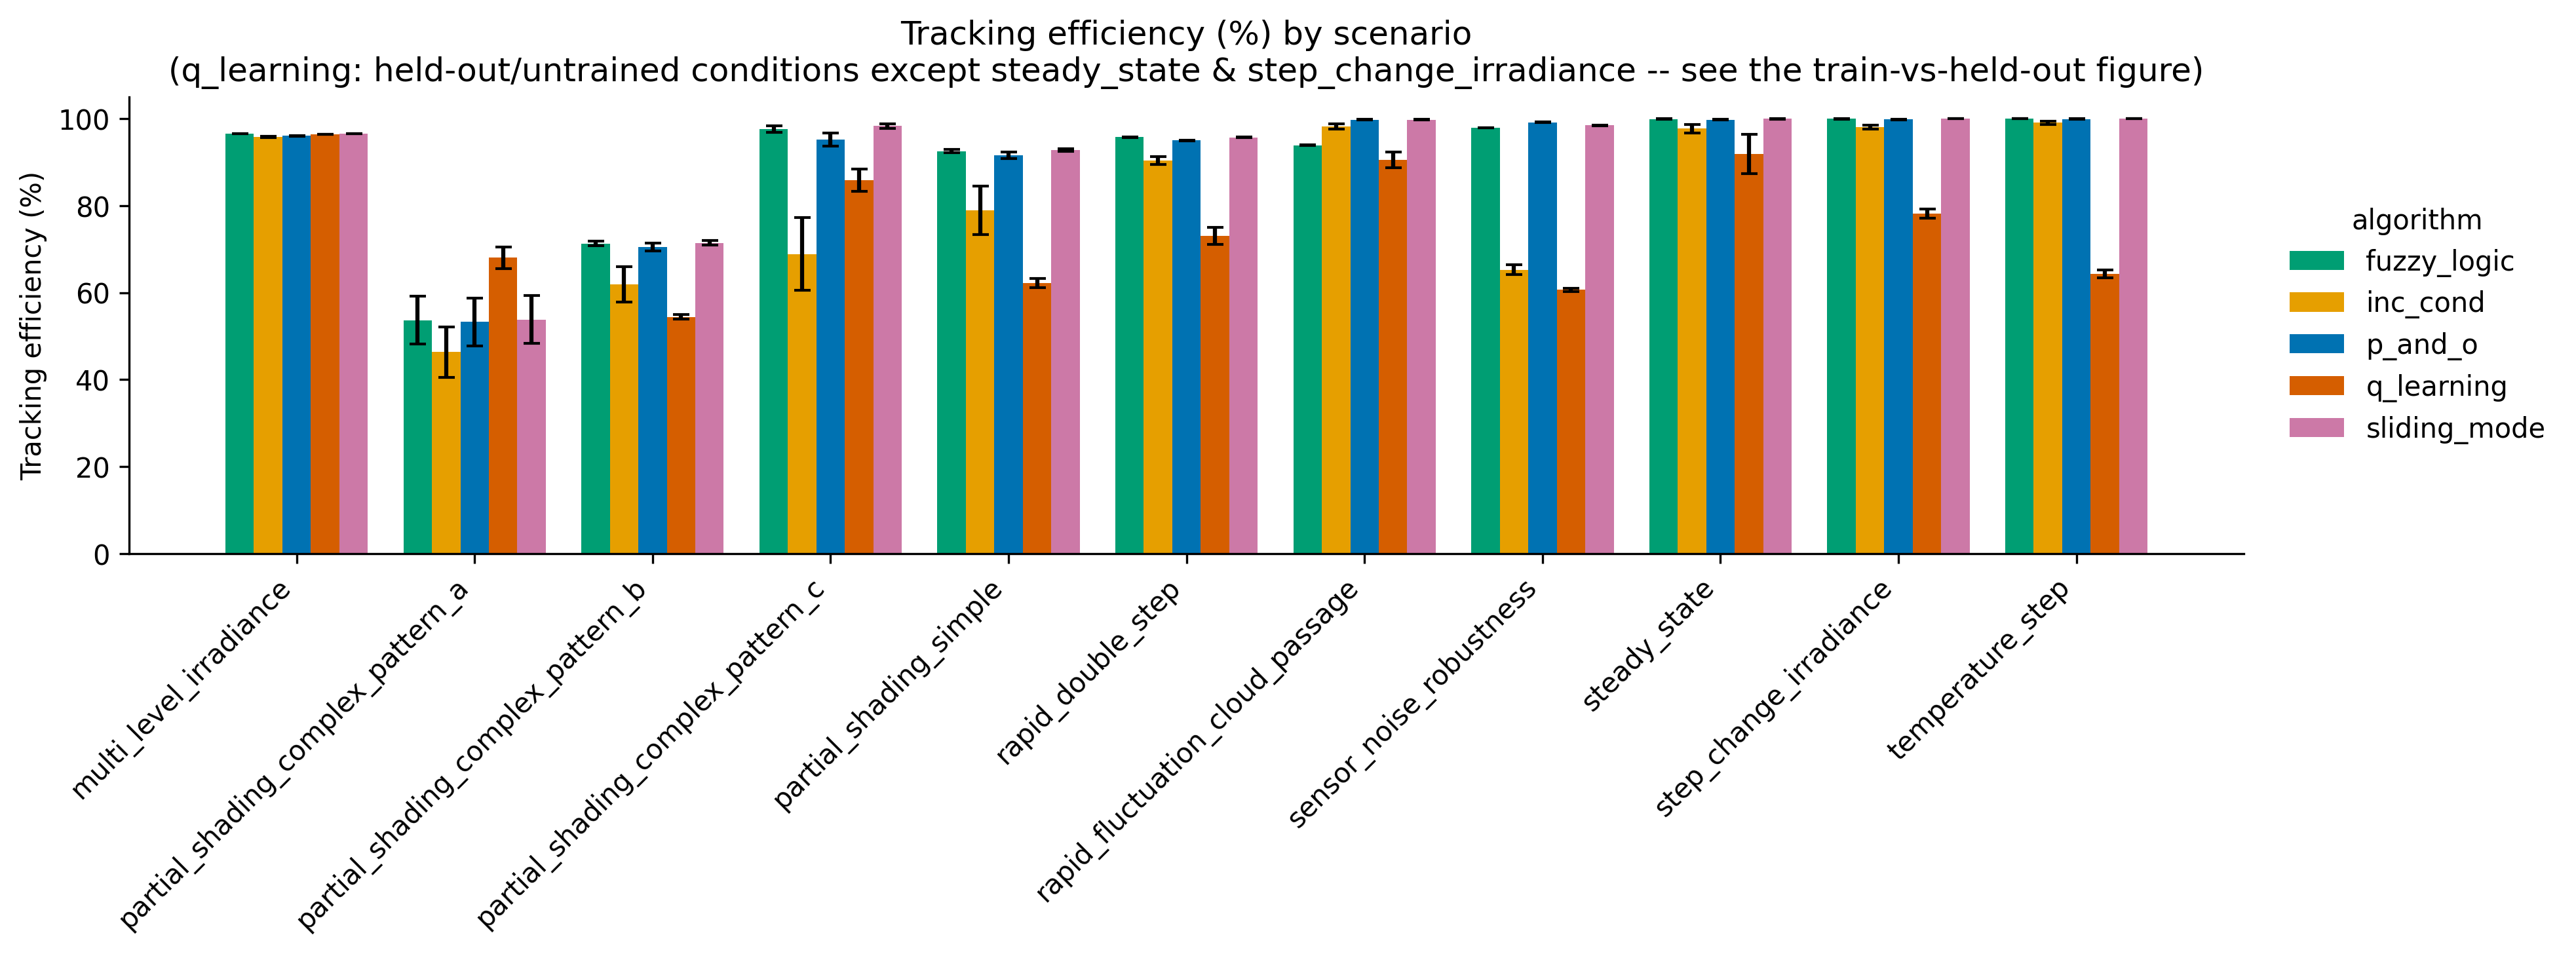
\includegraphics[width=\linewidth]{../results/figures/metric_comparison_tracking_efficiency_pct.png}
\caption{Tracking efficiency (\%) by scenario, all five core algorithms.
Q-learning's bars reflect held-out (untrained) conditions except at
\emph{steady\_state} and \emph{step\_change\_irradiance}; see
Fig.~\ref{fig:ql-train-held-out} for its dedicated train-vs-held-out
comparison.}
\label{fig:metric-comparison}
\end{figure}

\subsection{Partial Shading: A Shared Failure Across All Four Paradigms}
\label{sec:partial-shading-results}
Table~\ref{tab:convergence} reports \emph{convergence rate} -- the
fraction of the 50 Monte Carlo runs reaching within 2\% of the true global
MPP -- for all five core algorithms across all eleven scenarios. The
result is unambiguous: every algorithm, across all four paradigms,
achieves \textbf{0\% convergence} on three of the four partial-shading
configurations (\emph{simple}, \emph{Pattern A}, \emph{Pattern B}) --
uniformly zero, so an ANOVA/Friedman comparison would be degenerate there
(every group constant at 0\%; see the caveat in \texttt{src/analysis.py}'s
module docstring) and is not meaningful to report. Only \emph{Pattern C} --
the mildest configuration, with only two effective local maxima -- shows
partial success and, correspondingly, real cross-algorithm variance worth
testing: a one-way ANOVA on tracking efficiency is significant
($F=39.11$, $p=2.63\times10^{-25}$, $\eta^2=0.390$), and a Friedman test
agrees ($\chi^2=175.15$, $p=8.19\times10^{-37}$, $n=50$). Holm-corrected
paired $t$-tests confirm IncCond -- the only algorithm below 100\%
convergence here, at 44\% -- is significantly, and substantially, worse
than every other algorithm (vs.\ P\&O: $t=-7.71$,
$p_{\text{Holm}}=3.7\times10^{-9}$, $d=-1.09$; vs.\ fuzzy logic: $t=-7.59$,
$p_{\text{Holm}}=4.9\times10^{-9}$, $d=-1.07$; vs.\ SMC: $t=-7.56$,
$p_{\text{Holm}}=4.9\times10^{-9}$, $d=-1.07$; vs.\ Q-learning: $t=-5.78$,
$p_{\text{Holm}}=5.1\times10^{-7}$, $d=-0.82$) -- all large effect sizes,
confirming the 44\% convergence figure reflects a real, substantial
tracking-efficiency deficit rather than a handful of borderline runs
pulling a summary statistic down. Fig.~\ref{fig:convergence-heatmap} shows
the raw convergence-rate pattern across every scenario, not only the
partial-shading ones.

\begin{table}[htbp]
\centering
\caption{Convergence Rate (\% of 50 runs within 2\% of true MPP)}
\label{tab:convergence}
\begin{tabular}{@{}lccccc@{}}
\toprule
Scenario & P\&O & IncCond & Fuzzy & Q-learn.\ & SMC \\
\midrule
Steady state             & 100 & 70  & 100 & 80\textsuperscript{a} & 100 \\
Multi-level irradiance   & 100 & 100 & 100 & 100 & 100 \\
Step-change irradiance   & 100 & 100 & 100 & 100\textsuperscript{a} & 100 \\
Rapid double step        & 100 & 100 & 100 & 80  & 100 \\
Temperature step         & 100 & 100 & 100 & 80  & 100 \\
Rapid fluctuation        & 100 & 100 & 100 & 100 & 100 \\
Sensor noise             & 100 & 70  & 100 & 70  & 100 \\
Shading (simple)         & \textbf{0} & \textbf{0} & \textbf{0} & \textbf{0} & \textbf{0} \\
Shading Pattern A        & \textbf{0} & \textbf{0} & \textbf{0} & \textbf{0} & \textbf{0} \\
Shading Pattern B        & \textbf{0} & \textbf{0} & \textbf{0} & \textbf{0} & \textbf{0} \\
Shading Pattern C        & 100 & 44  & 100 & 98 & 100 \\
\bottomrule
\multicolumn{6}{l}{\footnotesize\textsuperscript{a}Training-distribution scenario for Q-learning.}
\end{tabular}
\end{table}

\begin{figure}[htbp]
\centering
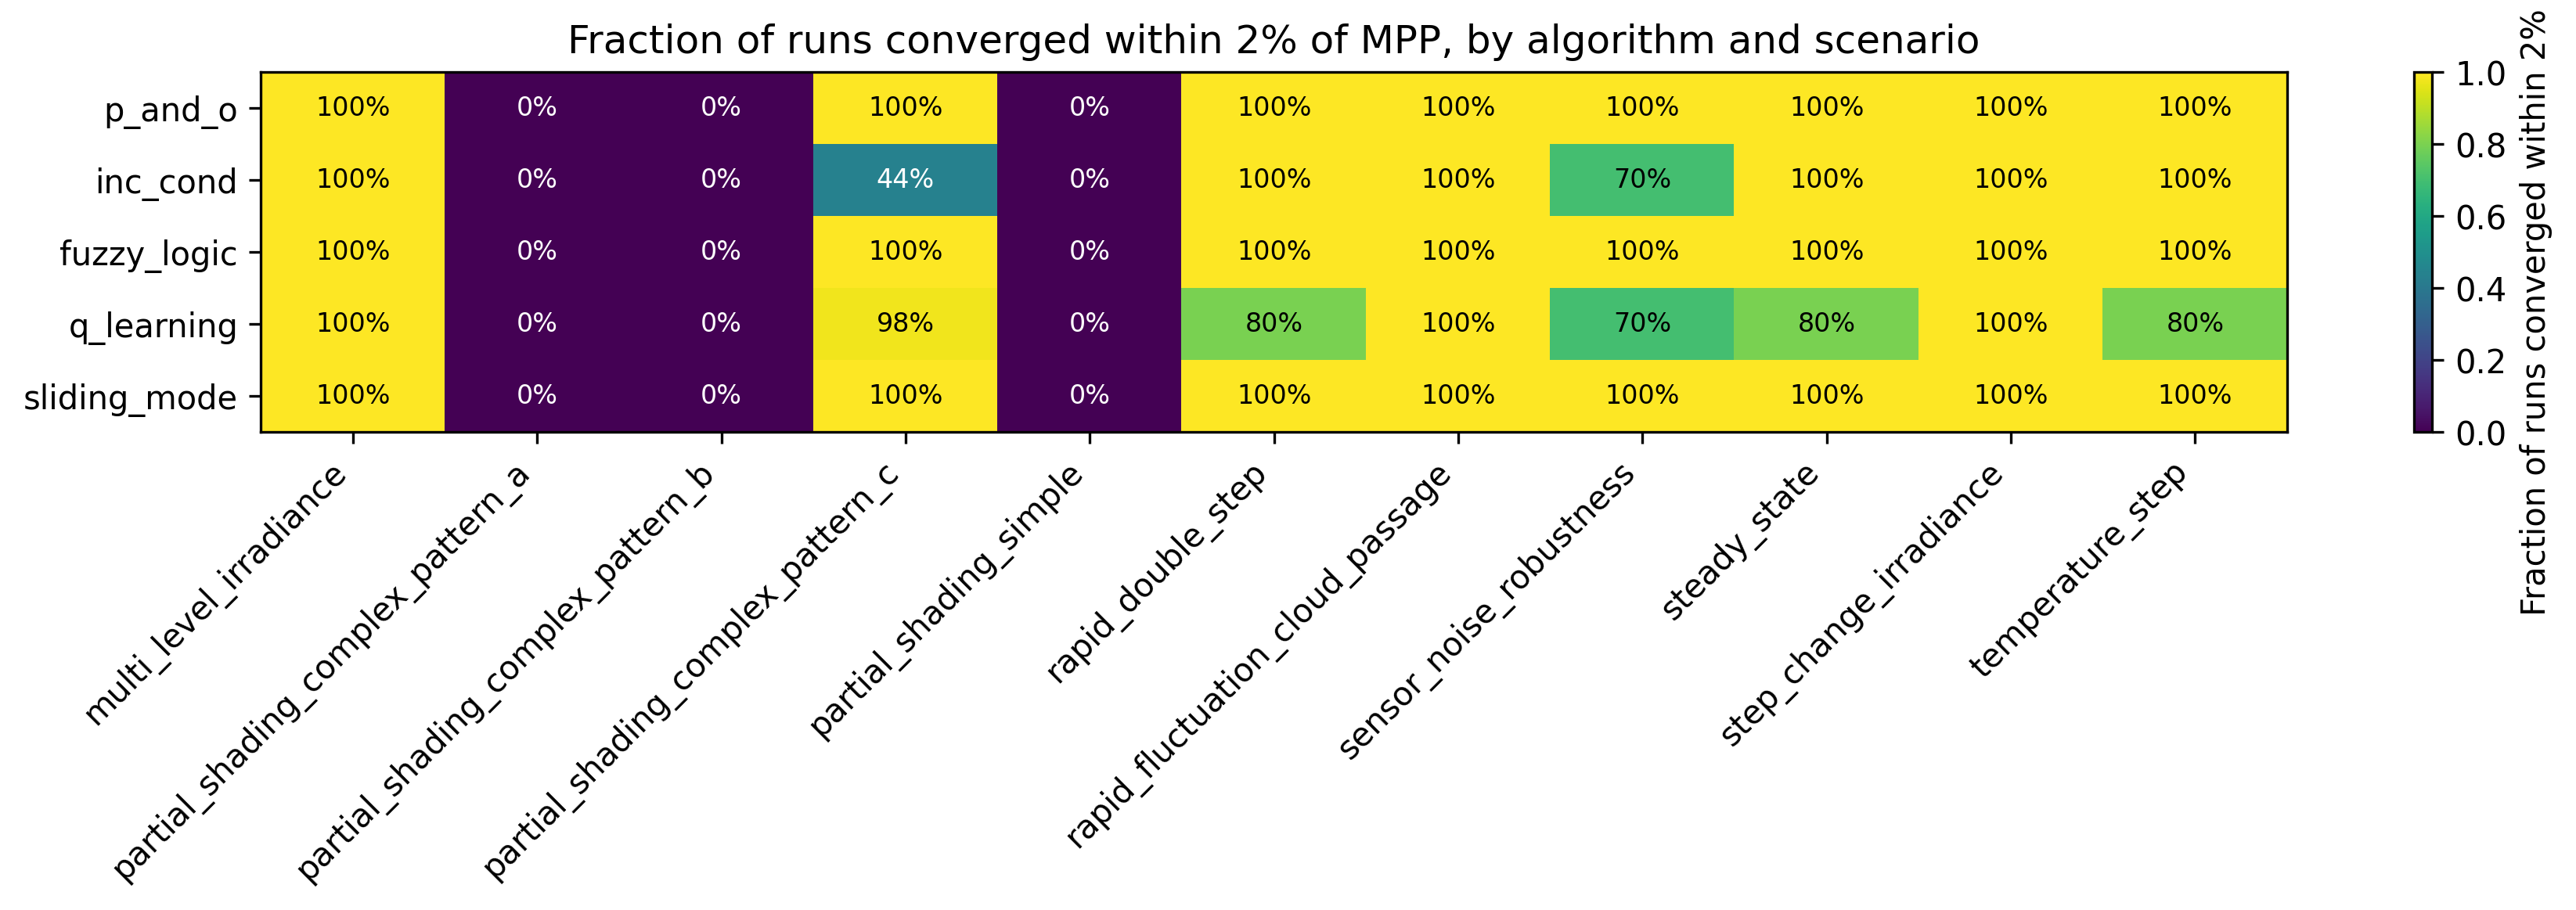
\includegraphics[width=\linewidth]{../results/figures/convergence_heatmap_convergence_rate.png}
\caption{Convergence rate (fraction of 50 runs reaching within 2\% of the
true MPP), algorithm $\times$ scenario. Colormap is \texttt{viridis}
(perceptually uniform, colorblind-safe), deliberately not a red-green
diverging map, which is exactly the wrong choice for the most common form
of color blindness.}
\label{fig:convergence-heatmap}
\end{figure}

\emph{Multi-level irradiance} originally showed a second, unrelated
0\%-convergence result for IncCond and SMC specifically, discovered during
this paper's own peer-review process and fixed prior to the results
reported here -- worth documenting because the mechanism is instructive.
At the scenario's lowest level (200\,W/m$^2$), the true MPP ($V=29.4\,$V,
$P=46.7\,$W) requires an effective source resistance
$R_{in}=V/I=18.6\,\Omega$ -- but a boost converter can only present
$R_{in}=R_{load}(1-D)^2 \le R_{load}=9.2\,\Omega$
(Section~\ref{sec:converter-model}), so this MPP is unreachable at
\emph{any} valid duty cycle, not merely one outside this paper's
$D\in[0.05,0.90]$ clamp range. Every algorithm's duty cycle is driven
toward the clamp floor while attempting to reach it. P\&O tolerates this
because it has no "hold" state at all -- every step perturbs, so it keeps
dithering right at the boundary until a perturbation away from it happens
to increase power. IncCond and SMC, by contrast, both use "no voltage
change between consecutive samples" as a proxy signal for being at or near
the MPP (IncCond's $dV\approx0$ boundary case; SMC's sliding surface
$s=dP/dV$, which reads exactly zero when $dV=0$) -- and being clamped at
the duty floor \emph{also} produces $dV\approx0$, for an entirely
different reason (the duty cycle simply cannot move, not because the MPP
condition is satisfied). Both algorithms' original implementations
misread this as convergence, locked in a zero correction, and never
attempted to move again even after irradiance later rose enough that the
true MPP became reachable. Since the only way to tell "clamped" apart from
"converged" is to actually try moving, both implementations now override a
hold (or a correction that would push further into a limit already
reached) with a small probe step away from that limit whenever duty is
already sitting at a bound -- using each algorithm's own existing
step/correction scale, so behavior away from a boundary, where "hold"
genuinely does mean converged, is unaffected. Table~\ref{tab:convergence}
reports the result after this fix: both algorithms now reach 100\%
convergence on this scenario, matching P\&O, fuzzy logic, and Q-learning,
confirmed by direct trajectory re-inspection showing duty cycle actually
escaping the clamp at each irradiance transition rather than staying
frozen. See Section~\ref{sec:conclusion} for what this implies about the
other results in this paper.

Crucially, the \emph{mechanism} of failure differs by paradigm, and this
is the more informative result than the raw 0\% figure alone.
Fig.~\ref{fig:trajectory-shading} illustrates this for the
\emph{partial-shading-simple} scenario (two modules at 1000/400\,W/m$^2$;
true global MPP at $V=60.5\,$V, $P=206.4\,$W). P\&O, IncCond, fuzzy logic,
and SMC all converge to the \emph{same local maximum} ($\approx193\,$W,
$\sim6.5\%$ below the true global optimum) -- unsurprising, since all four
follow the local $dP/dV=0$ (or equivalent) condition and have no mechanism
to escape a local maximum once reached. Q-learning, which was never
trained on any multi-module configuration at all
(Section~\ref{sec:ql-tagging}), does something qualitatively
\emph{worse}: rather than converging to either maximum, it moves the
operating point to a low-power region ($\approx114\,$W, roughly 45\% below
even the local maximum the other four algorithms reach) and oscillates
there indefinitely. This is a materially different -- and more severe --
failure mode than "stuck at a local maximum." Reporting Q-learning's
held-out performance honestly, rather than only its training-distribution
numbers, is precisely what surfaces this: a real, qualitatively distinct
weakness rather than a merely quantitative one.

\begin{figure}[htbp]
\centering
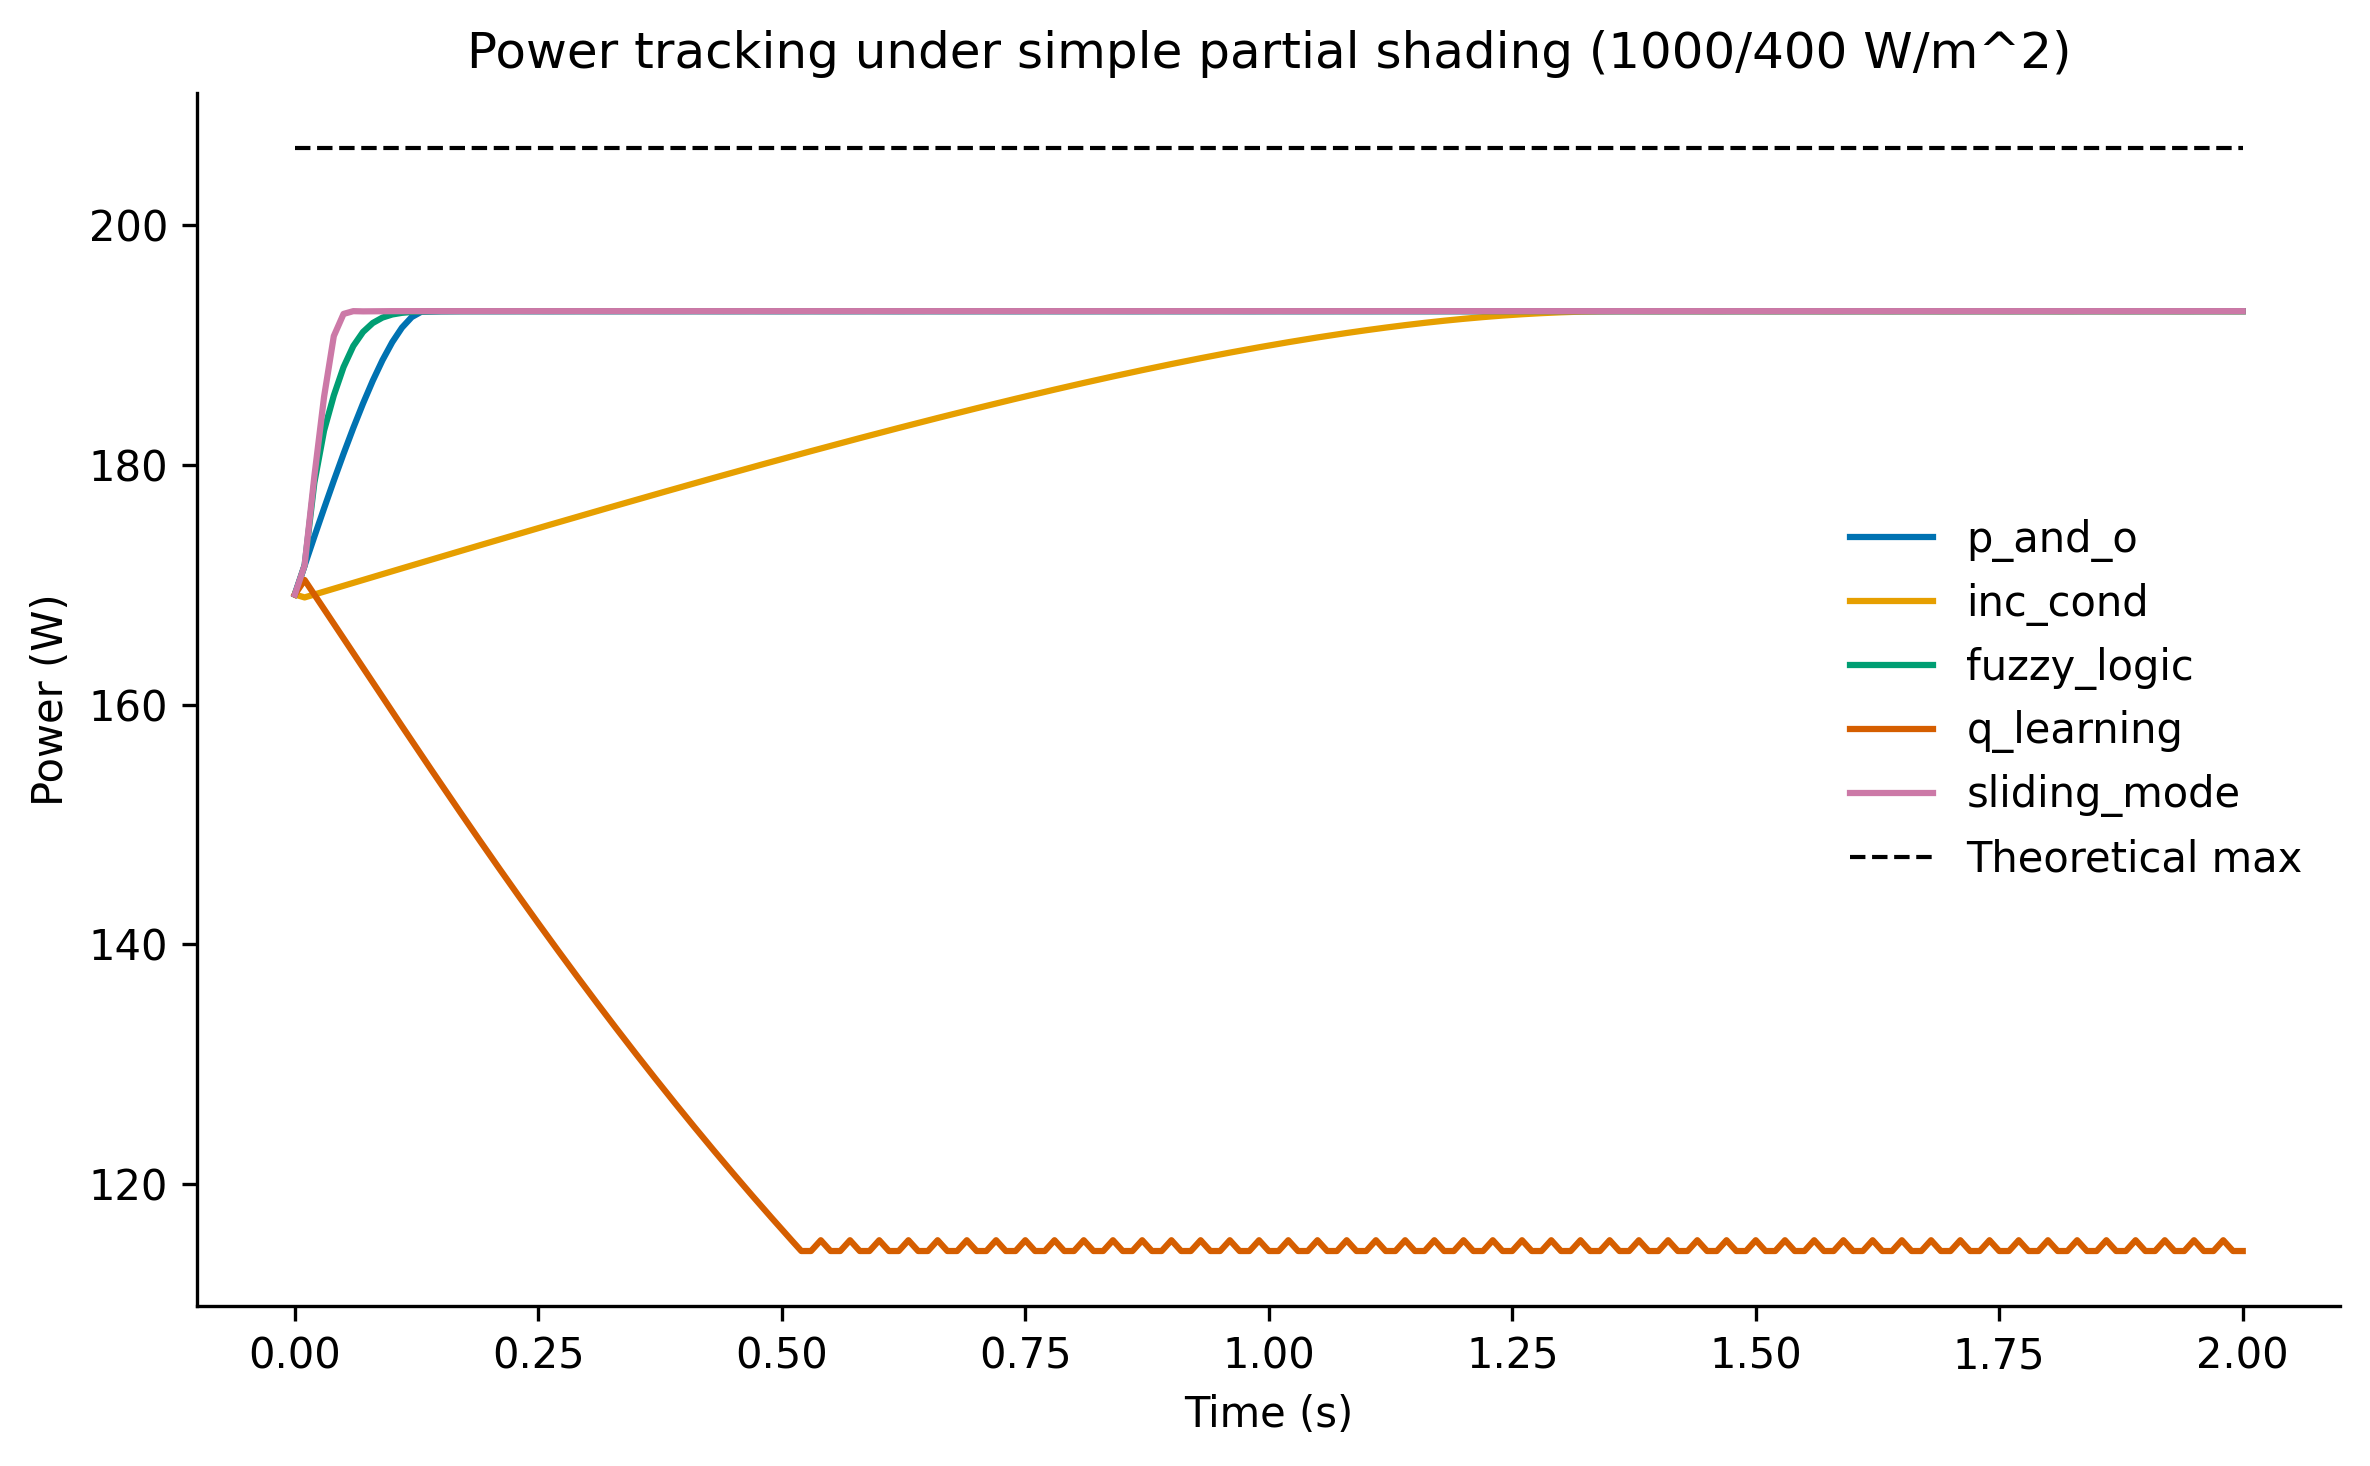
\includegraphics[width=\linewidth]{../results/figures/trajectory_partial_shading_simple.png}
\caption{Power tracking trajectories under simple partial shading
(1000/400\,W/m$^2$). P\&O, fuzzy logic, and SMC converge to a shared local
maximum ($\approx193\,$W); IncCond converges more slowly to the same
point; Q-learning (untrained on this topology) moves to and oscillates
around a lower-power operating point ($\approx114\,$W) instead.}
\label{fig:trajectory-shading}
\end{figure}

\subsection{Q-Learning: Train-Distribution vs.\ Held-Out}
Fig.~\ref{fig:ql-train-held-out} compares Q-learning's tracking efficiency
across all scenarios it was trained on versus all scenarios it was not,
per the tagging methodology in Section~\ref{sec:ql-tagging}. Consistent
with Section~\ref{sec:partial-shading-results}, the largest held-out gaps
occur under partial shading (a topology never seen in training, not merely
an unseen irradiance level), underscoring that this paper's train/held-out
split -- unlike flat-irradiance-only held-out evaluation -- is
specifically designed to expose a generalization failure that a
same-topology-only evaluation would miss entirely.

Notably, \emph{temperature\_step} -- a single-dimension change (temperature
only, same single-module topology, same irradiance) rather than a
topology change -- produces a held-out tracking efficiency of only
$64.3\%$, comparable in severity to two of the four partial-shading
patterns and well below every other held-out scenario except
\emph{sensor\_noise\_robustness} and \emph{partial\_shading\_simple}. This
is not merely an unseen-condition penalty: convergence rate for this
scenario is unchanged from before the temperature-step-away portion of the
run (80\%, identical to the other held-out scenarios' pre-step behavior),
but tracking efficiency collapses because the agent enters sustained,
large-amplitude oscillation after the 25$\to$50\textdegree C step
(steady-state oscillation p2p rises from a few watts to $\sim$100\,W) --
consistent with its fixed voltage-bin discretization
(Section~\ref{sec:q-learning-algorithm}), calibrated only against
STC-temperature operating ranges, placing the post-step operating point in
a state region the training distribution never adequately explored. This
strengthens, rather than merely restates, this paper's central
generalization finding: even a single-dimension shift outside the training
distribution -- not only a full topology change -- is enough to produce a
severe, qualitatively distinct failure mode for the tabular Q-learning
design used here.

\begin{figure}[htbp]
\centering
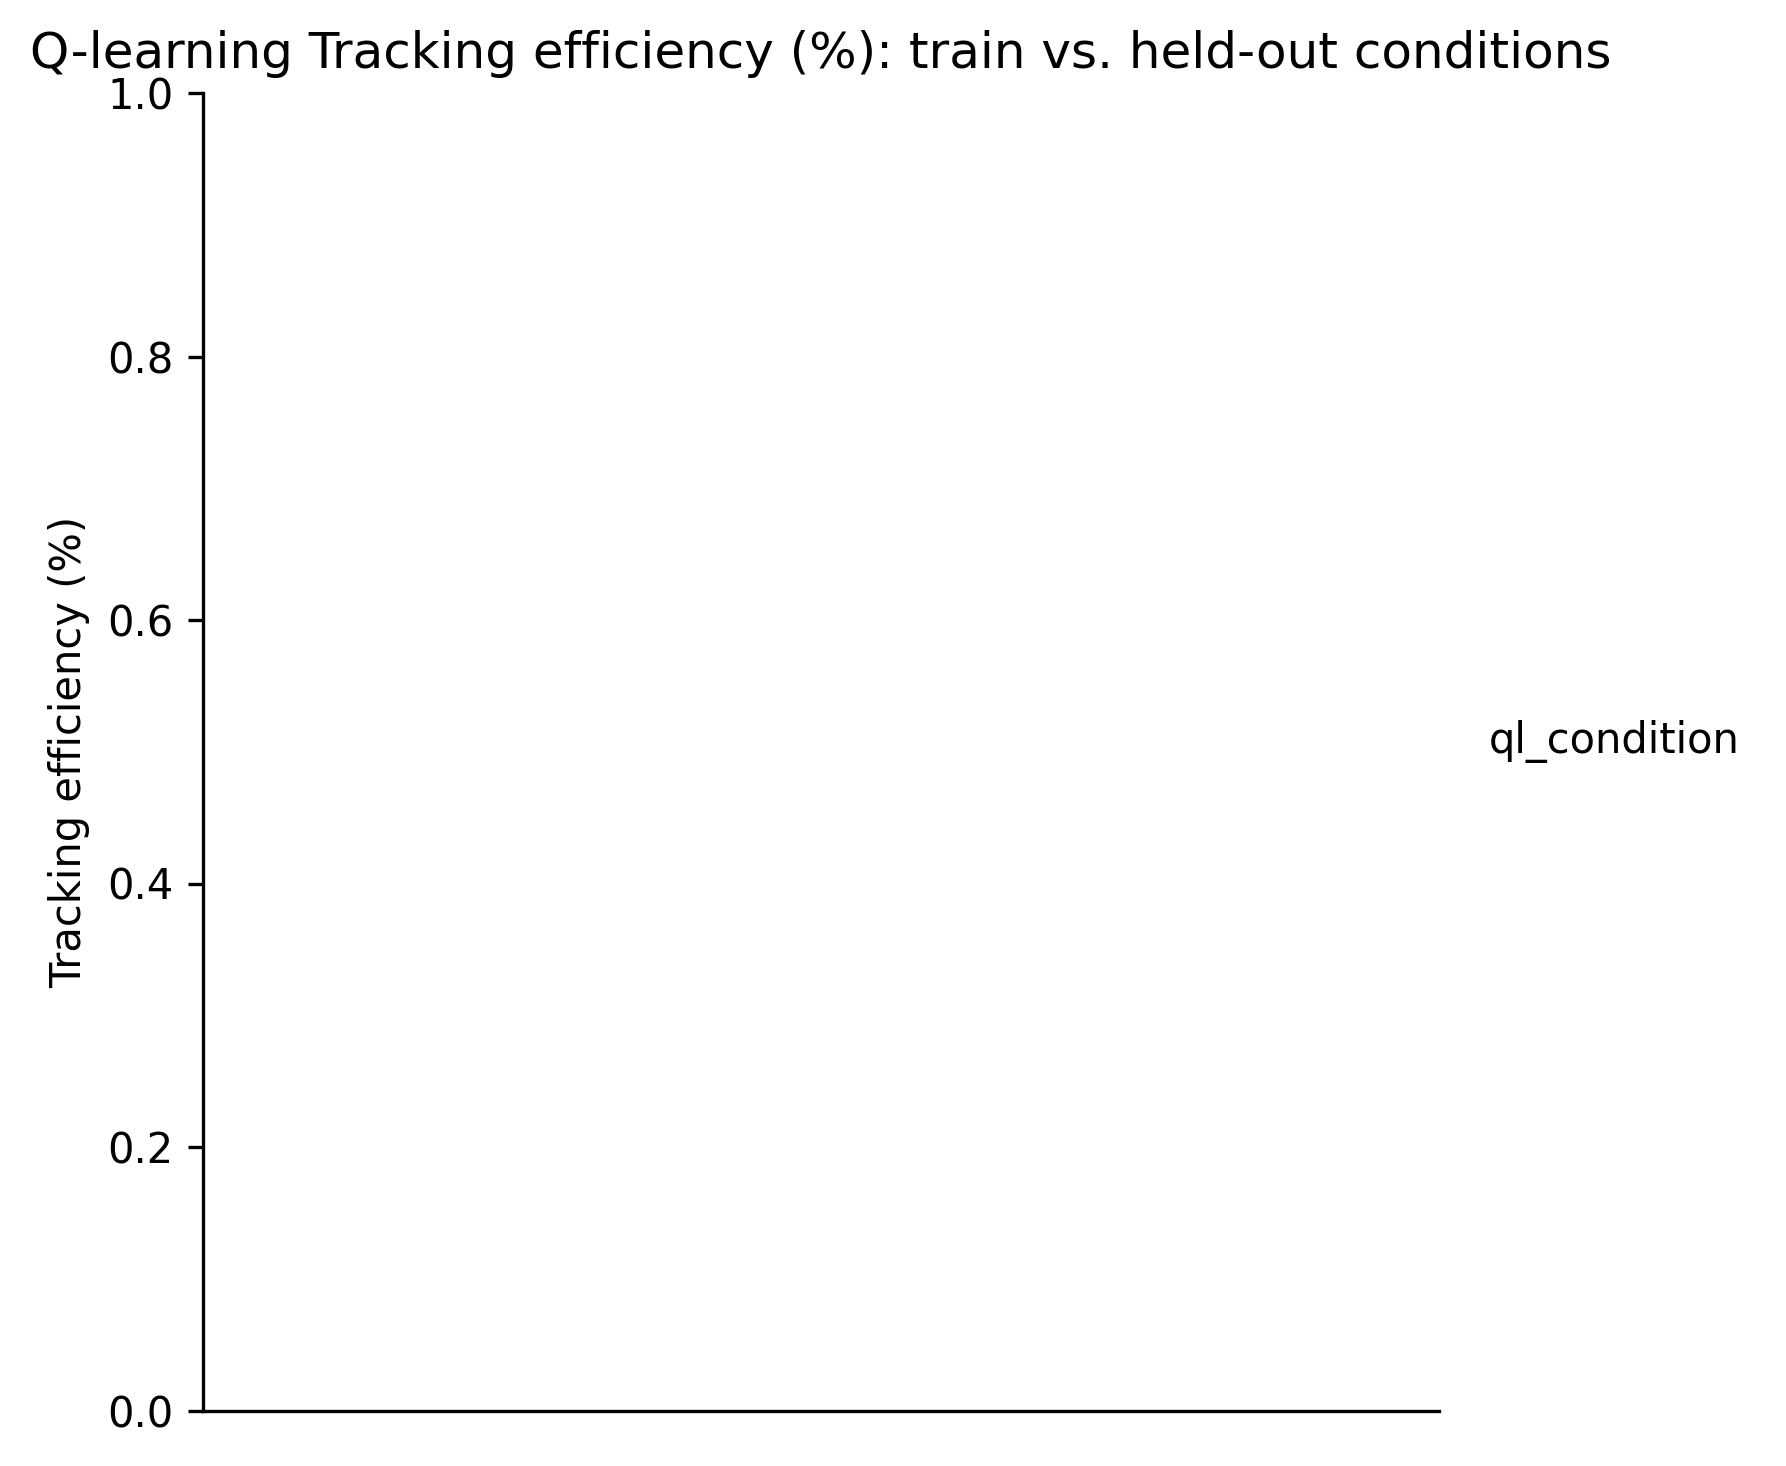
\includegraphics[width=\linewidth]{../results/figures/ql_train_vs_held_out_tracking_efficiency_pct.png}
\caption{Q-learning tracking efficiency (\%), grouped by whether the
scenario's conditions matched its training distribution.}
\label{fig:ql-train-held-out}
\end{figure}

\subsection{Fuzzy Rule-Base Sensitivity}
Table~\ref{tab:fuzzy-sensitivity} reports steady-state tracking efficiency
for the full $7\times7$ rule base against reduced $5\times5$ and
$3\times3$ variants (Section~\ref{sec:algorithms}). The $5\times5$
variant's 95\% confidence interval ($[99.83, 99.93]$) overlaps almost
entirely with the full $7\times7$ base's ($[99.82, 99.92]$) -- but
overlapping CIs are not the same claim as "statistically
indistinguishable," and a direct test shows they are not: a one-way ANOVA
across all three variants is significant ($F=16.38$, $p=3.77\times10^{-7}$,
$\eta^2=0.182$), a Friedman test agrees ($\chi^2=76.44$,
$p=2.52\times10^{-17}$, $n=50$), and the Holm-corrected paired $t$-test
between $7\times7$ and $5\times5$ specifically is itself significant
($t=-4.05$, $p_{\text{Holm}}=1.8\times10^{-4}$, $d=-0.57$, a medium effect
by convention). With $n=50$ paired samples, even the $0.01$ percentage
point gap between $99.87\%$ and $99.88\%$ reaches significance -- so the
correct claim is not "indistinguishable" but "a real, medium-sized effect
that is nonetheless practically negligible at the percentage-point level,"
a materially more precise version of the "reduced rule base matches full
performance" contribution this sensitivity analysis was designed to test.
The $3\times3$ variant is a clearer story: measurably lower ($99.01\%$, CI
$[98.58, 99.43]$) and a larger effect against both other variants (vs.\
$7\times7$: $t=4.65$, $p_{\text{Holm}}=7.7\times10^{-5}$, $d=0.66$; vs.\
$5\times5$: $t=4.64$, $p_{\text{Holm}}=7.7\times10^{-5}$, $d=0.66$). This
result has direct practical relevance given the computational-burden
finding below: fuzzy logic's $49$-rule Mamdani inference is measured at
roughly $101\times$ P\&O's per-step cost (Table~\ref{tab:burden}), so a
rule-base reduction that preserves performance at a practical, if not
perfectly statistical, level directly reduces that overhead.
Fig.~\ref{fig:fuzzy-sensitivity} shows the full per-scenario comparison,
not only the steady-state figures quoted above.

\begin{table}[htbp]
\centering
\caption{Fuzzy Rule-Base Sensitivity: Steady-State Tracking Efficiency (\%)}
\label{tab:fuzzy-sensitivity}
\begin{tabular}{@{}lccc@{}}
\toprule
Rule Base & Mean & 95\% CI \\
\midrule
$3\times3$ & 99.01 & [98.58, 99.43] \\
$5\times5$ & 99.88 & [99.83, 99.93] \\
$7\times7$ (full) & 99.87 & [99.82, 99.92] \\
\bottomrule
\end{tabular}
\end{table}

\begin{figure}[htbp]
\centering
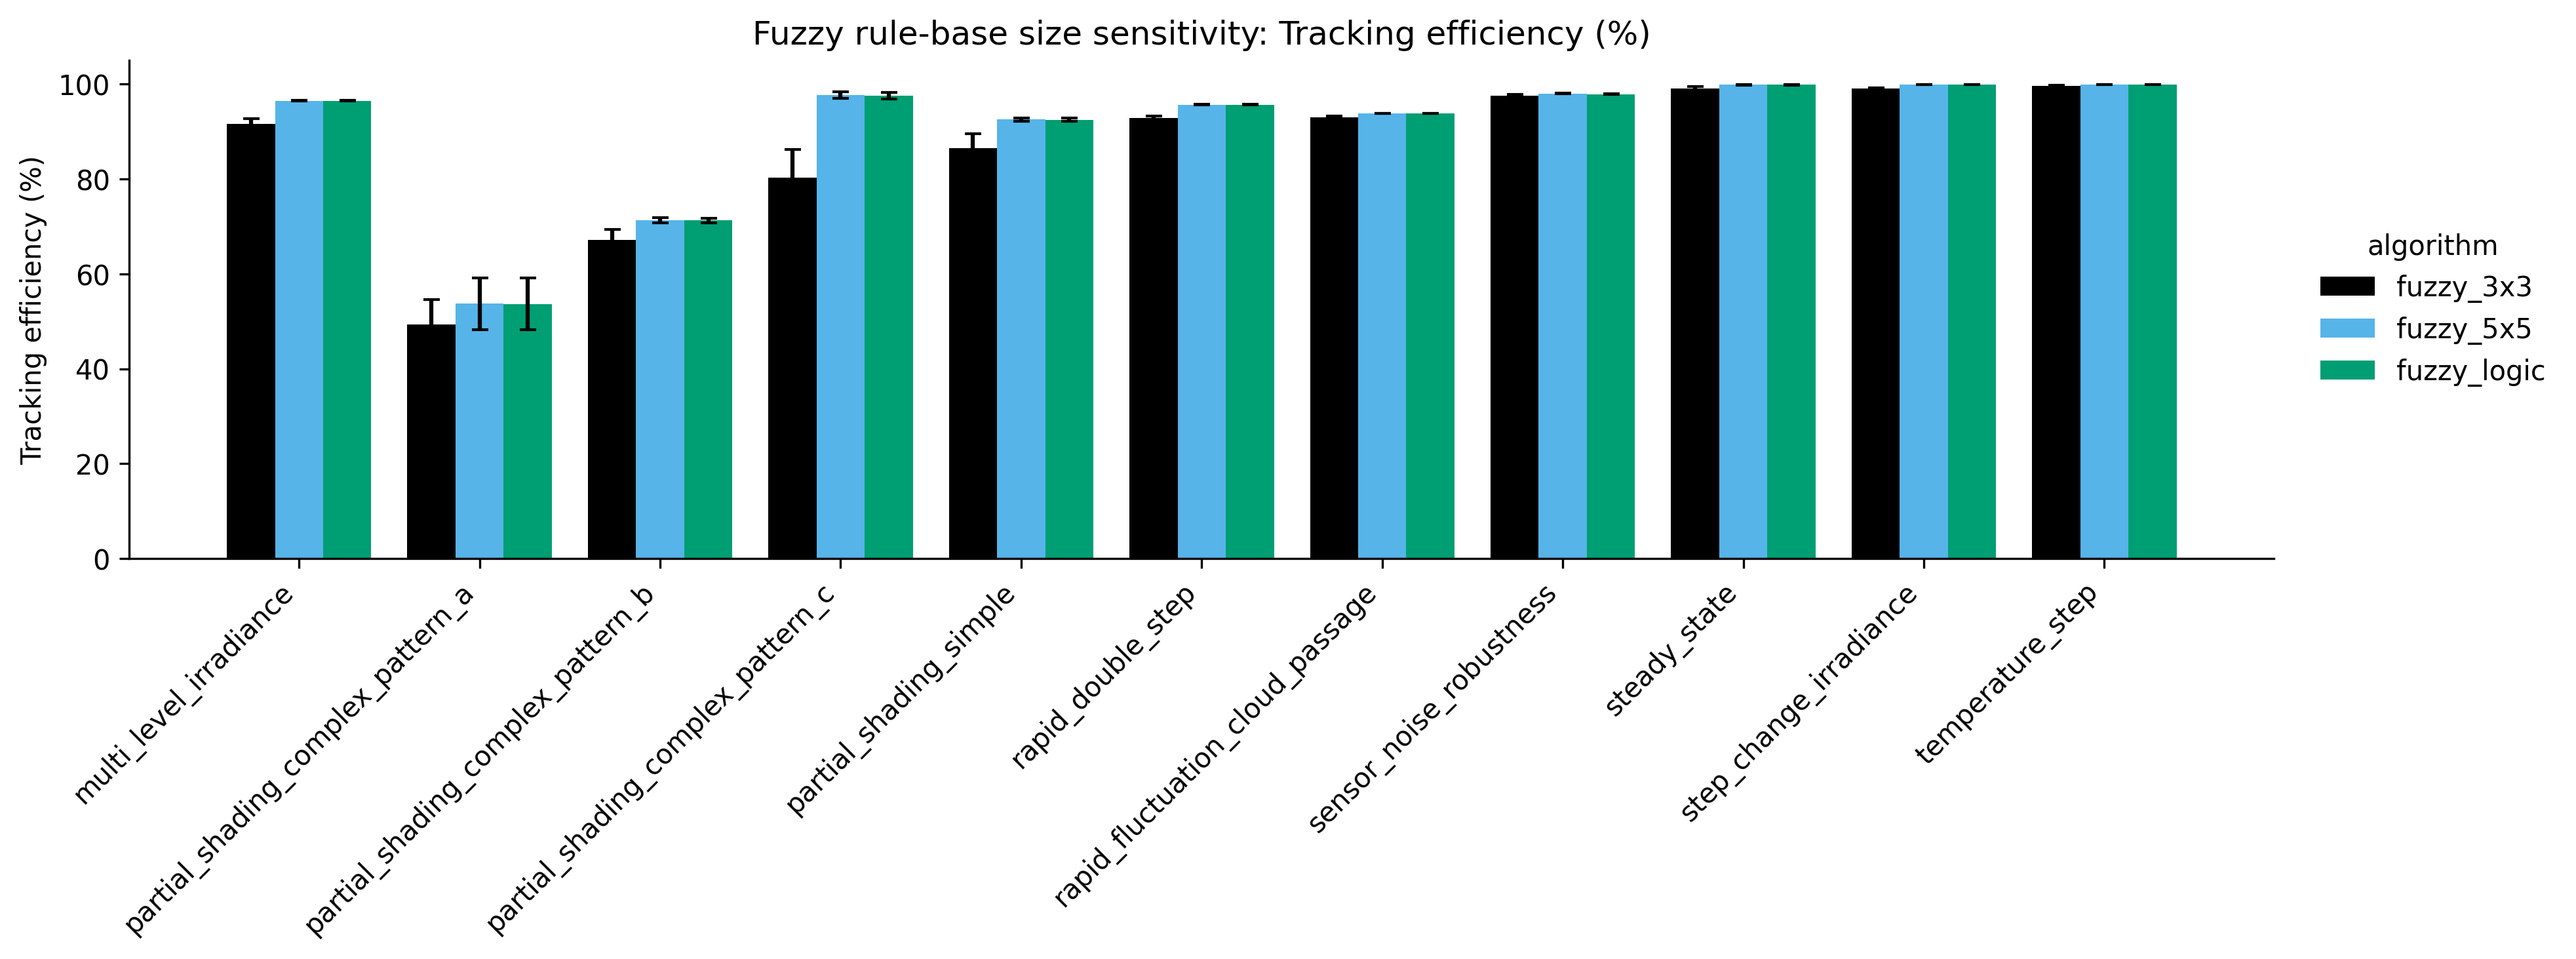
\includegraphics[width=\linewidth]{../results/figures/fuzzy_sensitivity_tracking_efficiency_pct.png}
\caption{Fuzzy rule-base size sensitivity: tracking efficiency (\%) across
all eleven scenarios, $3\times3$ vs.\ $5\times5$ vs.\ full $7\times7$.}
\label{fig:fuzzy-sensitivity}
\end{figure}

\subsection{Computational Burden}
\label{sec:computational-burden}
Table~\ref{tab:burden} reports mean per-\texttt{step()} wall-clock time,
normalized to P\&O. Fuzzy logic's Mamdani inference and centroid
defuzzification over a 201-point grid make it roughly two orders of
magnitude more expensive than P\&O; Q-learning's table lookup is
substantially cheaper than fuzzy logic but still an order of magnitude
above P\&O, reflecting per-step NumPy discretization overhead rather than
the lookup itself. IncCond remains close to P\&O's baseline cost; SMC is
somewhat above it, the extra cost of the boundary-clamp check added in
Section~\ref{sec:partial-shading-results}, as Fig.~\ref{fig:computational-burden}
shows directly. Wall-clock time is a
practical, deployment-relevant metric, but it conflates algorithmic
complexity with implementation detail (NumPy vectorization overhead,
Python interpreter cost, and run-to-run timing variance -- SMC's
measurement here is more sensitive to that variance than the others',
since its per-step cost is small in absolute terms) that an
operation-count or FLOP-based metric would isolate; we report wall-clock
time here because it is what a real embedded MPPT controller's
sample-period budget actually constrains, but treat the relative
orders-of-magnitude (not the exact multipliers) as the robust takeaway.

\begin{table}[htbp]
\centering
\caption{Computational Burden (Relative to P\&O = 1.0)}
\label{tab:burden}
\begin{tabular}{@{}lc@{}}
\toprule
Algorithm & Relative Burden \\
\midrule
P\&O         & 1.00 \\
IncCond      & 0.77 \\
SMC          & 1.61 \\
Q-learning   & 10.86 \\
Fuzzy Logic  & 101.26 \\
\bottomrule
\end{tabular}
\end{table}

\begin{figure}[htbp]
\centering
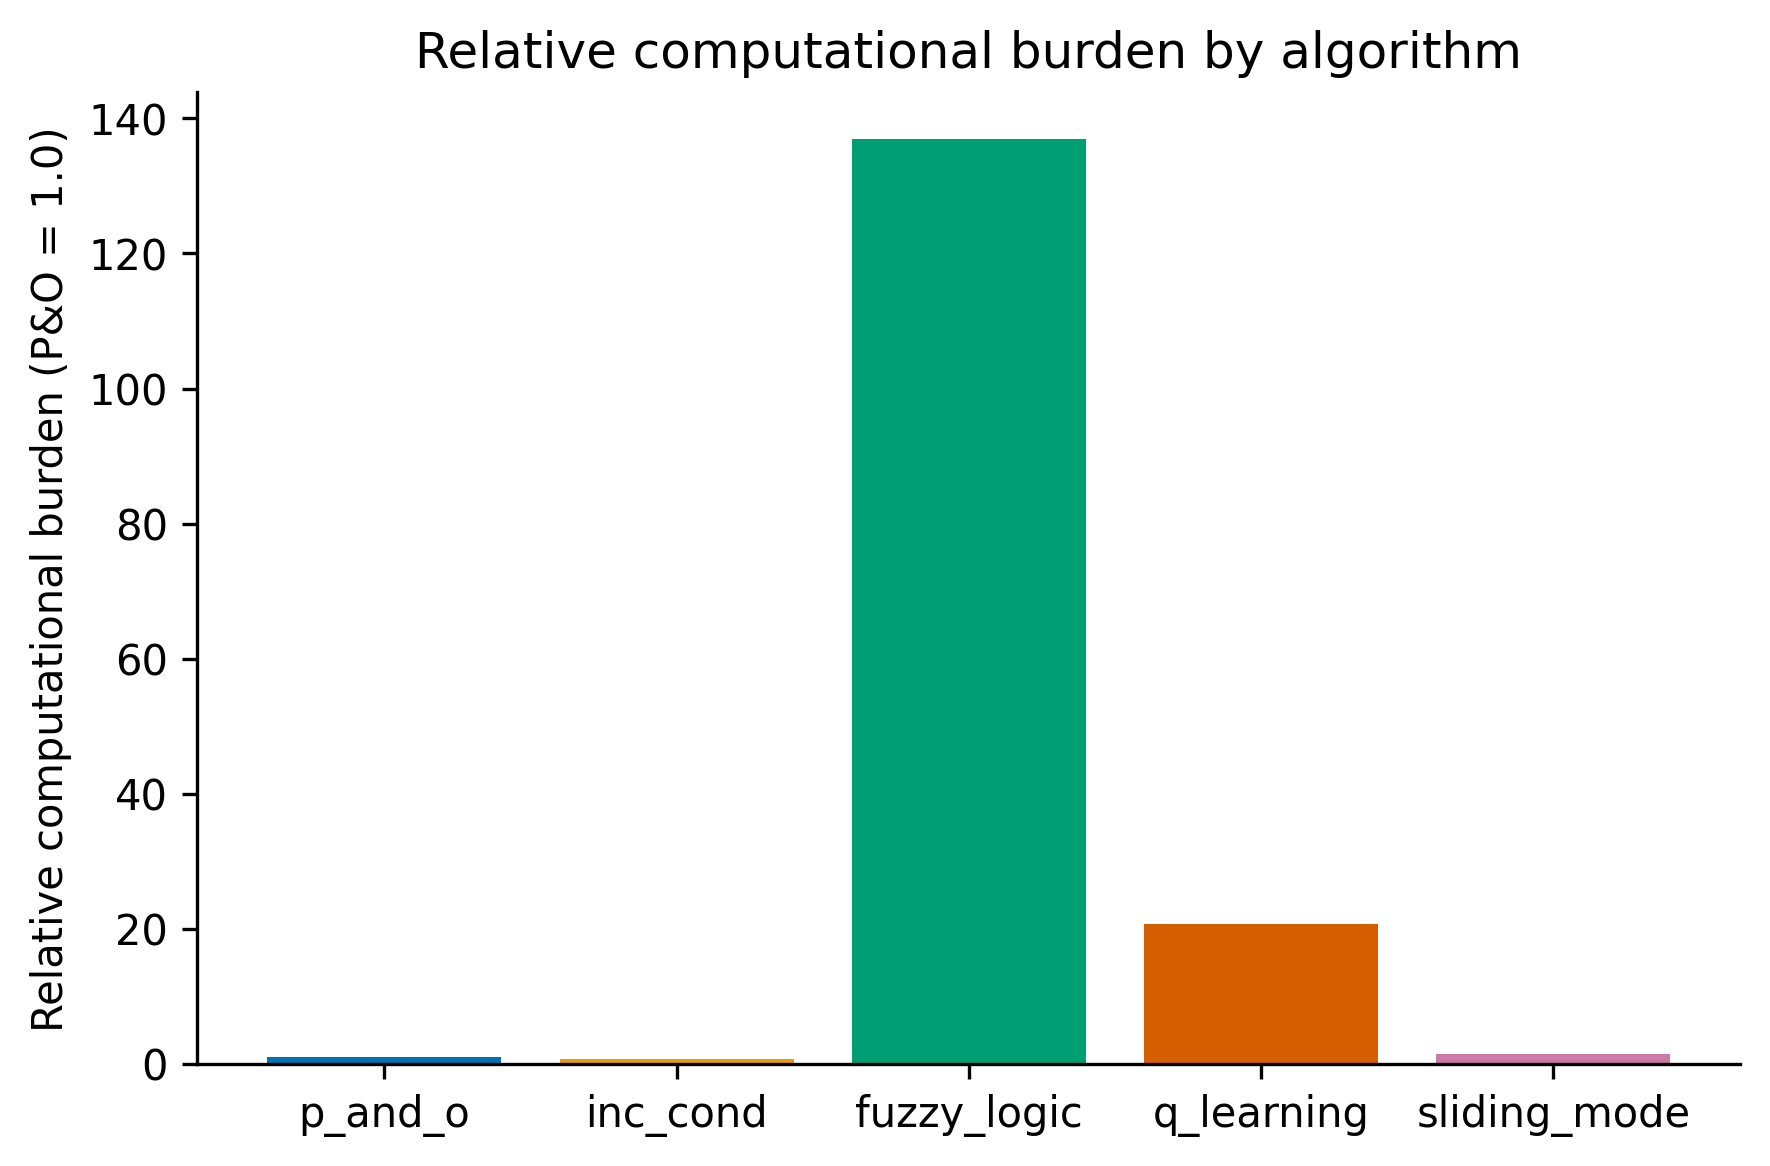
\includegraphics[width=\linewidth]{../results/figures/computational_burden.png}
\caption{Relative computational burden by algorithm (P\&O = 1.0).}
\label{fig:computational-burden}
\end{figure}

\subsection{Summary}
No single algorithm dominates across every scenario and metric: SMC gives
the best steady-state tracking efficiency and lowest oscillation at a
computational cost still well below the fuzzy and learning-based
paradigms, but it (and every other algorithm,
regardless of paradigm) fails to find the true global MPP under all but
the mildest partial-shading pattern tested. Fuzzy logic's rule-reduction
result is a genuine, statistically-supported contribution, but its
absolute computational cost remains two orders of magnitude above the
perturbative baselines even after reduction. Q-learning's generalization
failure under partial shading is qualitatively worse than the other
paradigms' local-maximum failures, a direct consequence of its training
distribution never including multi-module shading -- and the same fixed
discretization is fragile even to a single-dimension held-out condition
(temperature), not only a topology change, as Section~\ref{sec:results}'s
train-vs-held-out comparison shows. See Section~\ref{sec:conclusion} for
the limitations this implies.
